\documentclass[11pt, a4paper, oneside]{article}
\usepackage[a4paper,top=3cm,bottom=3cm,left=3cm,right=3cm]{geometry}
\usepackage{cite}
\usepackage[show]{ed}
\renewcommand{\familydefault}{\sfdefault}
\usepackage{helvet}
\usepackage{url}
\usepackage{parskip}		%% blank lines between paragraphs, no indent
\usepackage[pdftex]{graphicx}	%% include graphics, preferrably pdf
\usepackage{wrapfig}
\usepackage{xspace}
\usepackage[pdftex]{hyperref}	%% many PDF options can be set here
\usepackage{float} %%Use to put figures at an exact spot
\pdfadjustspacing=1		%% force LaTeX-like character spacing
\bibliographystyle{unsrt}
\newcommand{\myname}{Alexandru Valentin Toader}
\newcommand{\mytitle}{Space Filling Curve Index}
\newcommand{\latex}{\LaTeX\xspace}
\newcommand{\tex}{\TeX\xspace}
\newcommand{\mytodo}[1]{\emph{{\color{red} #1 \\}}}
\newcommand{\rplus}{R$^+$-tree$\,$}
\newcommand{\rstar}{R$^*$-tree$\,$}
\newcommand{\bplus}{B$^+$-tree$\,$}
\usepackage{nameref}
\usepackage{verbatim}
\usepackage{amsfonts}
\usepackage{amsmath}
\usepackage{graphicx}
\usepackage{gensymb}
\usepackage{rotating}

\hypersetup{
  pdfauthor = {\myname},
  pdftitle = {\mytitle},
  pdfkeywords = {},
  colorlinks = {false}
}

\begin{document}

  \pagenumbering{roman}

  \thispagestyle{empty}

  \begin{flushright}
   
\includegraphics[scale=0.7]{bsc-logo}
  \end{flushright}
  \vspace{20mm}
  \begin{center}
    \huge
    \textbf{\mytitle}
  \end{center}
  \vspace*{4mm}
  \begin{center}
   \Large by
  \end{center}
  \vspace*{4mm}
  \begin{center}
    \Large
    \textbf{\myname}
  \end{center}
  \vspace*{20mm}
  \begin{center}
    \large
    Big Data Project
  \end{center}
  \vfill
  \vspace*{8mm}
  \begin{flushleft}
    \large
    Date of Submission: \today \\
    \rule{\textwidth}{1pt}
  \end{flushleft}
  \begin{center}
    \Large Jacobs University --- School of Engineering and Science
  \end{center}

  \newpage


\newpage
\tableofcontents

\clearpage
\pagenumbering{arabic}

\section{Introduction}
%1. Array database intro
%2. 

Array database management systems (DBMS) offer scalable, flexible storage, and fast manipulation of n-dimensional homogeneous collections of items (array/raster data). Often, arrays are used to represent sensor, simulation, image or statistics data. 

There are many applications that benefit from efficient processing of array data such as: remote sensing, geology, oceanography, business data and gene data. These applications pose high requirements concerning the data and the operations that need to be supported, and therefore new techniques and tools are needed for increased processing efficiency.

One of the main issues that arise when working with high dimensional, terabyte objects is how to store them in the underlying system while maintaining a high level of performance. Due to their size, raster objects need to be divided into sub-arrays that can be easily managed by the underlying storage provider. In order to attain this, a system for indexing and retrieving fragments of n-dimensional objects must be provided.

Rasdaman is the leading array DMBS and has been used in applications involving data ranging from 1-D measurements to 4-D ocean and climate data. The rasdaman system partitions raster objects into tiles\cite{DBLP:conf/icde/FurtadoB99} which are indexed using a mechanism based on the \rplus. The individual tiles can be considered n-dimensional spatial objects (rectangles). 

The purpose of this project was to design and implement an indexing mechanism for multidimensional data objects using the Hilbert R-Tree as the underlying data structure.

The B+ tree\cite{Comer:1979:UB:356770.356776} has found wide adoption in the field of relational databases and represents the standard data structure for database index development. The task of storing, indexing and querying n-dimensional data is not well supported by indexes based on the B+ tree. 

The R-tree, proposed by Antonin Guttman\cite{Guttman:1984:RDI:602259.602266}, is the preferred method for indexing spatial data. The key idea is to group objects using their minimum bounding rectangle(MBR). Objects are added to a MBR within the node that will lead to the smallest increase in its size. The performance of R-trees depends on the quality of the algorithm that clusters the data rectangles on a node.

The \rplus is a compromise between R-trees and kd-trees: it avoids overlapping of internal nodes by inserting an object into multiple leaves if necessary. The \rplus offers increased point query performance over the original R-tree at the cost of a higher space utilization. 

The original R-tree, proposed by Guttman, is the basis of a number of variations and improvements\cite{Manolopoulos:2005:RTA:1098699}. The \rstar is considered the most robust variant, and has found numerous applications, in both research and commercial systems. However, the empirical study performed in \cite{Kamel:1994:HRI:645920.673001} has shown that the Hilbert R-Tree can perform better than the other variants in some cases.

Hilbert R-trees use the Hilbert space-filling curve to impose a linear ordering on the data rectangles with the goal of obtaining an improved clustering of the spatial objects.

To the extent of my knowledge, there is no open-source C++ implementation of the Hilbert R-tree data structure and providing one will be of great value to the community.

The initial specification for the project outlined the following objectives:
\begin{itemize}
\item Implement the Hilbert R-tree data structure
\item Create a benchmark to compare the performance of the indexing mechanism of the rasdaman system with a new Hilbert R-tree based implementation
\item Integrate the Hilbert R-tree data structure into the rasdaman database system.
\end{itemize}

The first two tasks have been successfully completed, while the third and last task has been left for future research.

The remainder of this document is structured as follows: section \ref{sec:related} discusses the theoretical foundations and algorithms necessary for the implementation of the Hilbert R-tree while also shortly describing the original R-tree implementation and the \rplus based implementation used in rasdaman, section \ref{sec:hrtree} describes in detail the technical details of the Hilbert R-tree implementation, followed by a technical description of the benchmark procedure in section \ref{sec:benchmark}.

The report ends with a discussion of the results and future work.

\section{Related work}
\label{sec:related}

In this section, I will first describe the original R-tree proposed by Guttman, as it lays the foundation for the \rplus data structure used in rasdaman and the Hilbert R-tree that is the subject of this project, followed by a short description of the \rplus variant of the R-tree used in rasdaman, a presentation of the Hilbert curve and, finally, a description of the Hilbert R-tree algorithm.

\subsection{R-tree}
The R-tree data structure was developed by Antonin Guttmann\cite{Guttman:1984:RDI:602259.602266} and is a hierarchical data structure based on the \bplus. It is used for the dynamic organization of a set of n-dimensional geometric objects represented by their n-dimensional minimum bounding rectangle. 

An R-tree of order $(m, M)$ has the following characteristics:
\begin{itemize}
\item Each leaf node (unless it is the root) can host at most $M$ and at least $m\leq \frac{M}{2}$ entries. Each entry is of the form $(mbr, oid)$, such that $mbr$ is the MBR that spatially contains the object and $oid$ is the object's identifier.
\item Each non-leaf node can store at most $M$ and at least $m\leq \frac{M}{2}$ entries. Each entry is of the form $(mbr, p)$ where $p$ is a pointer to a child of the node and $mbr$ is the MBR that spatially contains the minimum bounding rectangles contained in this child.
\item The minimum allowed number of entries in the root node is 2, unless it is a leaf (in this case, it may contain zero or a single entry)
\item All leaves of the R-tree are at the same level.
\end{itemize}

From the above definition, an R-tree is a height-balanced tree with a maximum height of $h_{max}=[log_mN]-1$ where $N$ is the number of data rectangles contained. The data structure is dynamic i.e. global reorganization is not required to handle insertions or deletions as we will see in the sub-section covering the insertion and deletion algorithms. 

It is worth mentioning that the MBRs of different nodes may overlap each other and a MBR can be contained (in the geometrical sense) in many nodes, but it can be associated to only one of them. This means that a query may visit many nodes before confirming the existence of a given MBR.

Two terms that are important for the performance of an R-tree are \textit{coverage} and \textit{overlap}. The coverage of a level of an R-tree is defined as the total area of all the rectangles associated with the nodes of that level. The overlap of a level of an R-tree is defined as the total area contained within two or more nodes. Efficient R-tree searching demands that both
overlap and coverage be minimized. Data structures based on the R-tree as the \rplus and the \rstar use methods that improve these two metrics. 

The R-tree supports the following operations: searching for objects whose MBR intersects a query rectangle $Q$, inserting new objects, and deleting existing objects.

\subsubsection*{Search}
Given a rectangle, $Q$, we can find all data rectangles that are intersected by this rectangle. The search starts from the root node of the tree. For every entry $(mbr, p)$ in a non-leaf node, if $mbr$ intersects $Q$, the search continues on the node that $p$ points to. When a leaf node is reached, Q is tested for intersection with each MBR of each leaf entry, and the entries that are intersected are returned.

\subsubsection*{Insertion}
Insertions in an R-tree are handled similarly to insertions in a \bplus. The R-tree is traversed to locate an appropriate leaf to insert the new entry. At each step, the rectangles in the current node are examined, and a candidate is chosen using a heuristic such as choosing the rectangle which requires the least enlargement. The search descends into the tree until a leaf node is found.

The entry is inserted in the found leaf and all nodes on the path from the root to that leaf are updated accordingly. If the leaf cannot accommodate the new entry because it is full, then it is split into two nodes.

In case of a split, the redistribution of the leaf entries is done following a heuristic which impacts the performance of the tree. The objective of the split algorithm is to minimize the probability of invoking both created nodes for the same query. 

Three different split algorithms have been proposed by Guttman: linear split, quadratic split and exponential split. Each algorithm trades efficiency of the split for time-complexity. The quadratic split is considered a good compromise between the quality of the split and the time-complexity of the algorithm.

\subsection*{Deletion}
In order to delete an entry from the R-tree, the search algorithm is used to find the entry which is then removed from the containing node. If the node does not underflow after the deletion, its parent nodes will be updated and the algorithm finishes. If an underflow takes place, the node in which the deletion took place is dissolved and its entries are reinserted.

\subsection{\rplus}

The standard R-Trees dynamic insertion algorithms might lead to a structure that has excessive space overlap and "dead-space" in the nodes which results in bad performance. Efficient R-tree searching demands that both overlap and coverage be minimized. It has been shown that zero overlap and coverage is only achievable for data points that are known in advance and, that using a packing technique for R-trees search is dramatically improved\cite{Roussopoulos85directspatial}.

The \rplus \cite{Sellis:1987:RDI:645914.671636} is a variation of Guttman's R-trees that avoids overlapping rectangles in intermediate nodes of the tree by allowing partitions to split rectangles. The paper introducing the data structure shows that the \rplus achieves up to 50\% savings in disk accesses compared to an R-tree when searching files of thousands of rectangles.

The entries of the \rplus are identical to the ones of the original R-Tree with the following extensions\cite{Sellis:1987:RDI:645914.671636}:
\begin{itemize}
\item For each entry $(p,mbr)$ in an intermediate node, the subtree rooted at the node pointed to
by $p$ contains a rectangle $R$ if and only if $R$ is covered by $mbr$. The only exception is when
$R$ is a rectangle at a leaf node; in that case $R$ must just overlap with $mbr$.

\item For any two entries $(p_1 , mbr_1 )$ and $(p_2, mbr_2)$ of an intermediate node, the overlap between $mbr_1$ and $mbr_2$ is zero.

\end{itemize}

One property satisfied by an R-tree but not by an \rplus is that in the former, every node contains between $M/2$ and $M$ entries unless it is the root. In consequence, the \rplus achieves better search performance at the expense of space utilization. In the case of point queries, the \rplus can achieve  even more than 50\% savings in disk accesses compared to the R-tree. The R-tree suffers in the case of few, large data objects, which force a lot of "forking" during the search while the \rplus handles these cases, by splitting these large data objects into smaller ones.

A full discussion of the \rplus algorithms and a performance comparison to the R-tree is available in \cite{Sellis:1987:RDI:645914.671636}. 

\subsection{Hilbert curve and compact Hilbert index}
%Describe space filling curves
A space-filling curve is a parametrized, injective function which maps a unit line segment to a continuous curve in a hypercube, which gets arbitrarily close to a given point in the hypercube as the parameter increases.\cite{MR1299533}. In essence, this means that space filling curves can be used for dimension reduction i.e. by using the inverse of the curve generating function, one can map a multidimensional point to a point on a line.

Space filling curves that are Lebesgue measure-preserving have the additional property that equal length intervals map to equal volumes i.e. points that are close together in 1-dimensional space will map to objects that are close together in multidimensional space.

The Z-order curve, the Hilbert curve, and the Gray-code curve\cite{Faloutsos:1988:GCP:53064.53065} are examples of space filling curves. In \cite{Faloutsos:1989:FSK:73721.73746}, it was shown experimentally that, given a set of n-dimensional rectangles, the Hilbert curve achieves the best clustering among the three methods above i.e. the rectangles that are close together in n-dimensional space will be mapped to points that are close together in 1-dimensional space.

The geometric construction of the Hilbert curve starts with the $\sqcap$ shape as shown in the first image of figure ~\ref{fig:hilbert}. This is known as an order 1 Hilbert curve. Given an order k curve, one can obtain an order k+1 curve as follows:
\begin{enumerate}
\item Place a copy of the curve, rotated $90\degree$ counter clock-wise, in the lower right.
\item Place a copy of the curve, rotated $90\degree$ clockwise, in the lower left.
\item Place a copy of the curve in the upper right and one in the upper left.
\item Connect the four disjoint curves.
\end{enumerate} 

The first six orders of the Hilbert curve can be seen in figure ~\ref{fig:hilbert}.

\begin{figure}[h!]
  \centering
    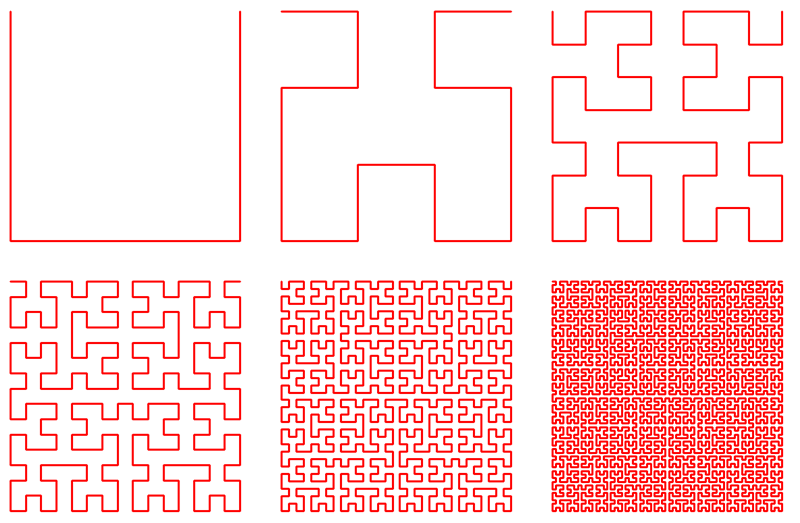
\includegraphics[width=0.9\textwidth]{img/Hilbert6}
    \caption{"Hilbert curve". Licensed under CC BY-SA 3.0 via Wikipedia add -  \protect\url{http://en.wikipedia.org/wiki/File:Hilbert_curve.svg\# mediaviewer/File:Hilbert_curve.svg}}
  \label{fig:hilbert}
\end{figure}


When the order of the curve tends to infinity, the resulting curve is a fractal, with a fractal dimension of 2. The Hilbert curve can be generalized for higher dimensions. The path of a space filling curve imposes a linear ordering on the grid points. Figure ~\ref{fig:hilbert-ordering} shows such an ordering for an order 2 curve. For example the point (0,0) on the curve has a Hilbert value of 0, while the point (1,1) has a Hilbert value of 2. 

\begin{figure}[h!]
  \centering
    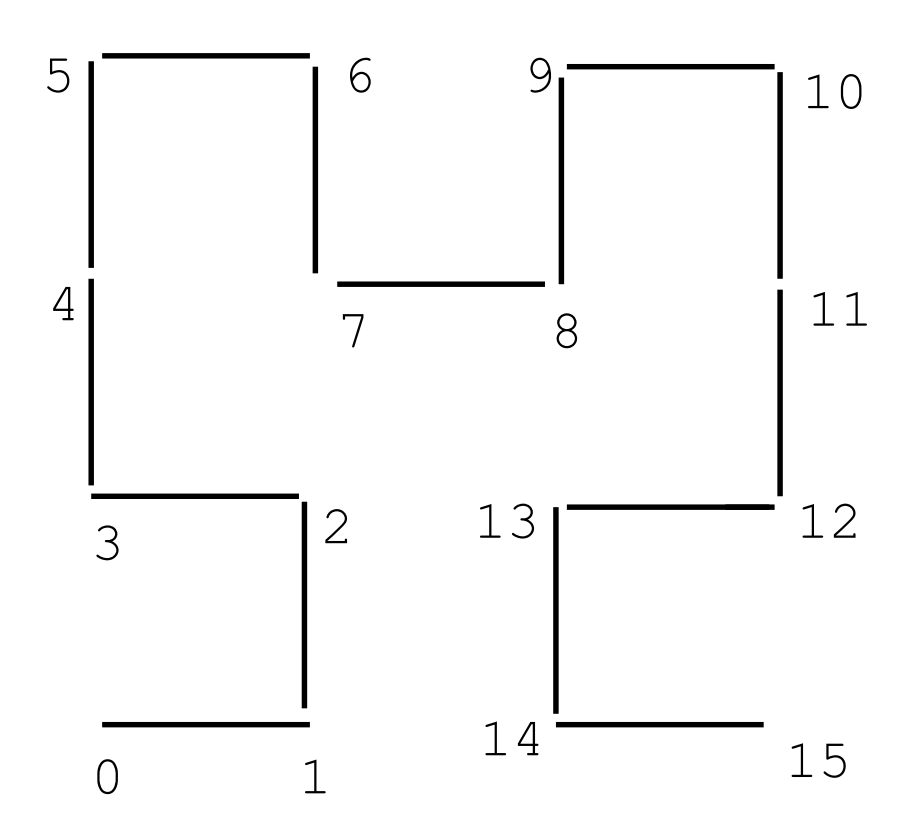
\includegraphics[width=0.5\textwidth]{img/HilbertOrdering}
    \caption{Ordering imposed by the Hilbert curve {\cite{Kamel:1994:HRI:645920.673001}} }
  \label{fig:hilbert-ordering}
\end{figure}

%Describe the compact hilbert index

A method for efficiently computing the Hilbert coordinates of a n-dimensional point is described by Hamilton and Rau-Chaplin in \cite{Hamilton:2008:CHI:1330769.1330914}. A C++ library based on this method is offered by Chris Hamilton at \url{https://web.cs.dal.ca/~chamilto/hilbert/}. Using this library I have implemented the Hilbert R-tree data structure described in the following subsection.

\subsection{Hilbert R-Tree}
A standard R-tree splits a node on overflow, turning 1 node into 2. The Hilbert R-Tree is a data structure, based on the original R-Tree, that offers the possibility of deferred splitting of overflowing nodes. This leads to better space utilization and better search performance.

A Hilbert R-tree of order $(m,M)$ has the following structure. A leaf node contains at least $m$ and at most $M$ entries of the form $(mbr, obj\_id, h)$ where $mbr$ and $obj\_id$ are the same as in the standard R-tree and $h$ is the Hilbert value associated with the center of $mbr$. A non-leaf node contains at least $m$ and at most $M$ entries of the form $(mbr, ptr, LHV)$ where $mbr$ and $ptr$ are the same as in the standard R-tree and $LHV$ is the largest Hilbert value among the data rectangles enclosed by $mbr$.

The Hilbert value of the entries is used to create an ordering on the nodes and leads to the concept of sibling nodes. As discussed in the previous subsection, this ordering groups similar data rectangles together, minimizing the area and the perimeter of the resulting minimum bounding rectangles.

By using the ordering imposed on the nodes of the Hilbert R-tree, instead of splitting a node that overflows into two nodes, we can implement an $s$ to $s+1$ splitting policy. In other words, when a node is overflowing, it tries to push some of its entries to $s-1$ of its siblings. If all the siblings are full, a new node is created and the entries of the $s$ nodes is distributed among the $s+1$ siblings. By adjusting the split policy, space utilization of the tree's nodes can be driven arbitrarily close to 100\%.

I will briefly describe the search, insert and delete procedures while referring the reader to the original paper on the Hilbert R-tree by Kamel and Faloutsos \cite{Kamel:1994:HRI:645920.673001} for a detailed explanation.

\subsubsection*{Search}
Given a query rectangle $Q$, the search procedure starts from the root and descends the tree examining all nodes that intersect the query rectangle. When the algorithm reaches a leaf, it reports all entries that intersect the query window $Q$ as results.

\subsubsection*{Insertion}
To insert a new rectangle $r$ in the Hilbert R-tree, the Hilbert value $h$ of the center of the new entry is used as key. 

The algorithm initially descends the tree to find a suitable leaf for the new entry. At each level, the node with the minimum LHV greater than the one of the new entry is chosen. When a leaf node is reached, the rectangle $r$ is inserted in the correct position according to $h$.

If the leaf is about to overflow, the entries are first distributed among the leaf's siblings. If all the $s$ cooperating siblings are about to overflow, a new node is created and the entries of the $s$ cooperating siblings are divided among the $s+1$ nodes. The LHV and MBR of the nodes directly affected by the insert are updated.

Finally, the changes are propagated upwards by adjusting the LHV and MBR of all the affected parent nodes.

\subsection*{Deletion}
In the Hilbert R-tree orphaned nodes do not need to be reinserted whenever a father node underflows. Instead of reinserting the node, we borrow keys from its cooperating siblings or, if all the siblings are about to underflow, the $s+1$ siblings are merged into $s$ siblings. Finally, the changes are propagated upwards towards the root.

The Hilbert R-tree provides a better space utilization and greater search performance than the other R-tree variants at the cost of a higher insertion cost. In the benchmarks displayed in \cite{Kamel:1994:HRI:645920.673001}, the Hilbert R-tree outperforms the \rstar and the standard R-tree in all tests.

In the next section I will give details about the C++ implementation of the Hilbert R-tree that was done for this project.

\section{Hilbert R-tree implementation}
\label{sec:hrtree}

\begin{sidewaysfigure}
  \centering
    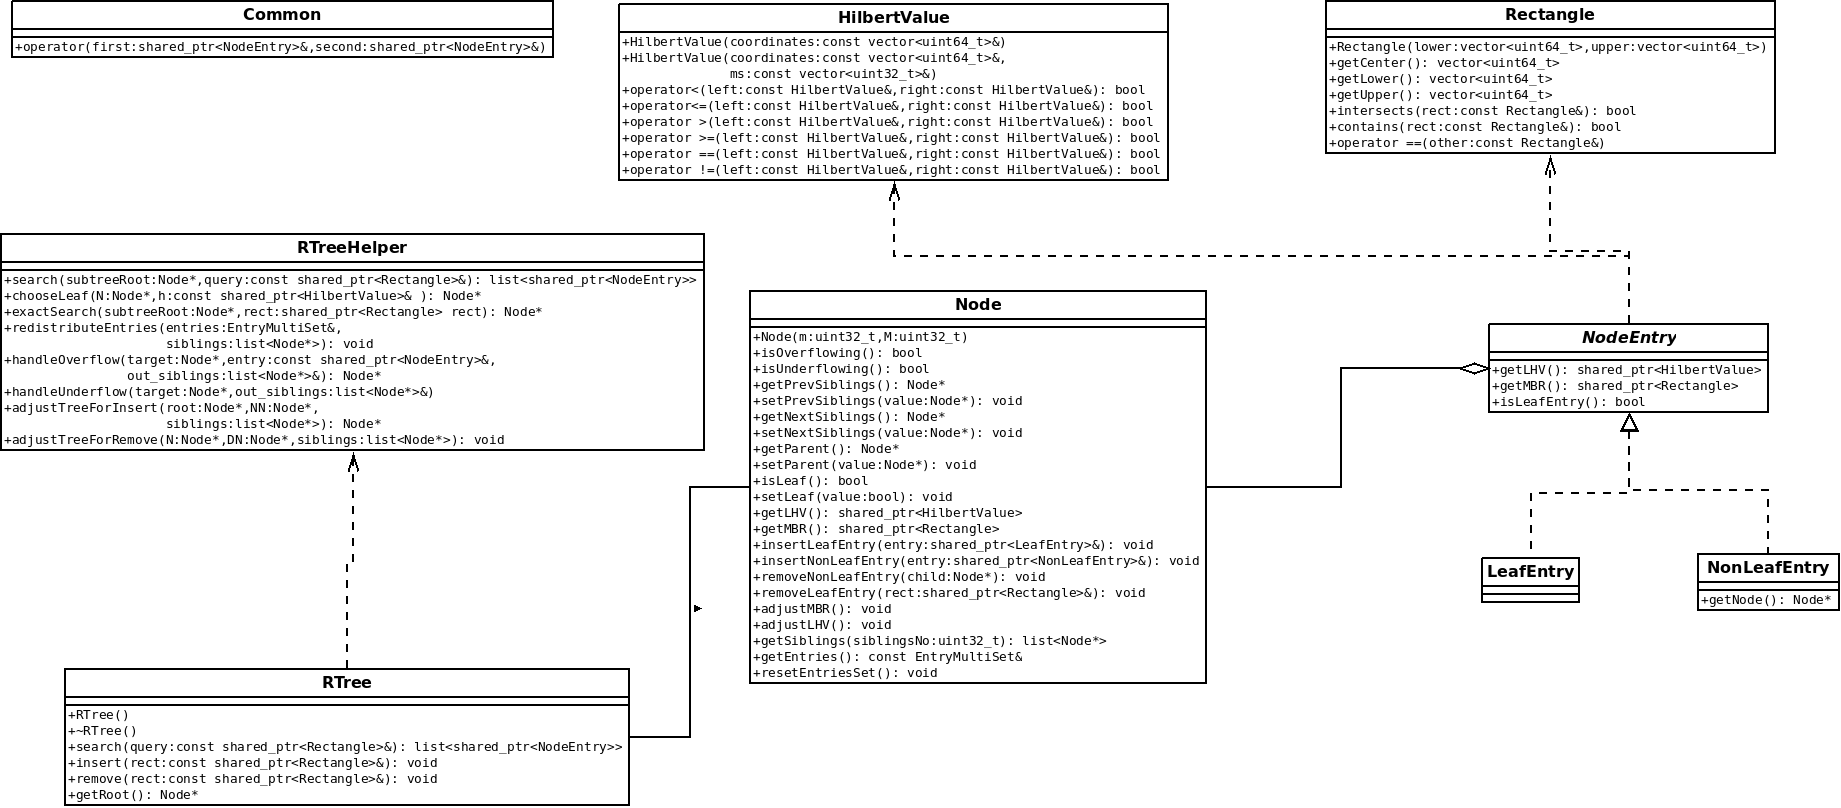
\includegraphics[width=0.9\textwidth]{img/ClassDiagram.png}
      \caption{Hilbert R-tree class diagram}
  \label{fig:class_diagram}
\end{sidewaysfigure}


The implementation of the Hilbert R-tree was performed in C++ using the Compact Hilbert Index library\cite{libhilbert} implemented by Chris Hamilton and the Boost library \cite{boost}.

The code was written following a test-driven development process. This lead to a large number of tests which also act as a secondary developer documentation for the code.
The class structure of the software can be seen in figure ~\ref{fig:class_diagram}.

To the extent of my knowledge, there is no implementation of the Hilbert R-tree for n-dimensional data available on the internet. The code written in this step is a basis for integration into the rasdaman index manager.

The implementation if very well tested and documented, and can be found here \url{https://github.com/atoader/HilbertRTree} together with instructions on how to build and run it.
\section{Benchmark implementation}
\label{sec:benchmark}
% What is the purpose of this benchmark?
In order to compare the performance of rasdaman's current indexing algorithm based on the \rplus with a new implementation based on the Hilbert R-tree, a benchmark was developed for this purpose.

The benchmark is comprised of a set of test cases which have been implemented in the array DBMS benchmarking framework developed by George Merticariu\cite{GM}.

% Where is the index used?
In rasdaman, raster objects are maintained in a standard relational database, based on the partitioning of an array object into tiles\cite{DBLP:conf/icde/FurtadoB99} ~\ref{fig:rasdaman-tile}. Tiles are stored as BLOBs. The indexing mechanism employed by rasdaman, which is the subject of a possible improvement through this research, is the component that manages these BLOBs.

\begin{figure}[h!]
  \centering
    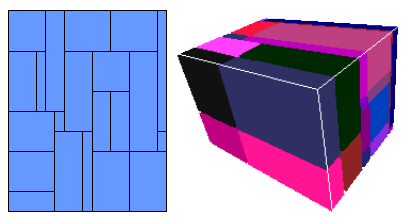
\includegraphics[width=0.9\textwidth]{img/tiling}
    \caption{"Sample tiling of an array for storage in rasdaman" by Pebau.grandauer - Licensed under CC BY-SA 3.0 via Wikimedia Commons -\url{http://commons.wikimedia.org/wiki/File:Sample_tiling_of_an_array_for_storage_in_rasdaman.png\# mediaviewer/File:Sample_tiling_of_an_array_for_storage_in_rasdaman.png }}
  \label{fig:rasdaman-tile}
\end{figure}

% What should it test?
Rasdaman offers a set of options that can be used to tune the tile storage to the user's requirements when inserting a new collection into the database:

\begin{verbatim}
INSERT INTO collName VALUES ...
[ TILING tilingName tilingOptions [ TILE SIZE tileSize ] ]
[ INDEX indexName ]
\end{verbatim}

These options have an impact on the performance of subsequent queries on the inserted data. The \textit{indexName} parameter is used to select the type of index and it will be used to distinguish between the \rplus implementation and the Hilbert R-tree implementation. The \textit{tileSize} parameter determines the size of a tile. The size of the tile determines the overall number of tiles and also influences how the data is stored on disk. The \textit{tilingName} option allows the user to select from a list of available tiling schemes. 

% What parameters are of importance for the test?
Because this benchmark assesses the performance of the component that indexes tiles and not of the tiling scheme, a regular tiling will be used. The tile size will be varied for the same collection, in order to measure its impact on the indexing performance.

% How should it test?
The benchmark is developed to verify the performance of the index manager from the DMBS user's point of view. Using the rasql component, queries will be run and timed through the mentioned benchmarking framework.

% What operations are performed?

 The trials described below will measure the performance of inserting new data into the index, searching data in the index and removing data from the index. To this end, the tests have been separated into three classes: Insertion, Search and Deletion. As the type of data that is indexed is of no importance to the performance of the index, random character data will be used.
 
\subsubsection*{Insertion}
In order to test the performance of insertion, I will create collections of dimension ranging from 1-D to 6-D, sizes of 1MB, 10MB, 100MB, 1GB and 10GB, and tile sizes of 1MB, 4MB and 16MB while using the regular tiling scheme.

\subsubsection*{Search}
In order to test the performance of search, for each of the collections inserted in the previous step, I have performed the following operations:
\begin{enumerate}
%\item  
\item Retrieve slices of the collection, centered at the upper-left corner and of increasing size in every dimension. This will test the performance of the indexing structure when a large number of nodes are processed by the search algorithm. An example for the 2-D case can be seen in figure ~\ref{fig:search1}.
\item Retrieve slices of the same dimension, positioned at sequential coordinates through the collection. An example for the 2-D case can be seen in figure ~\ref{fig:search2}. 
\item Retrieve multiple subsets of the collection at the same time.
\end{enumerate}

\begin{figure}[h!]
  \centering
    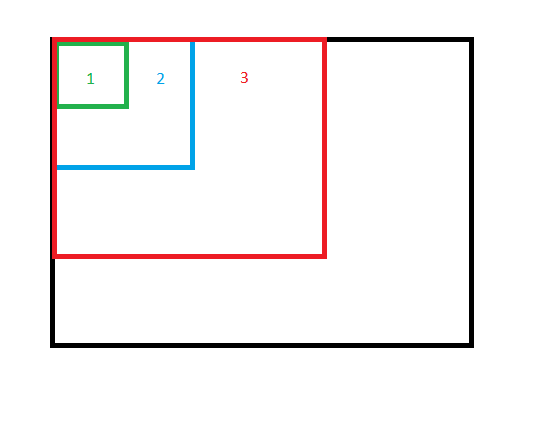
\includegraphics[width=0.5\textwidth]{img/search1}
      \caption{Sequential retrieval of increasing subsets of a collection}
  \label{fig:search1}
\end{figure}

\begin{figure}[h!]
  \centering
    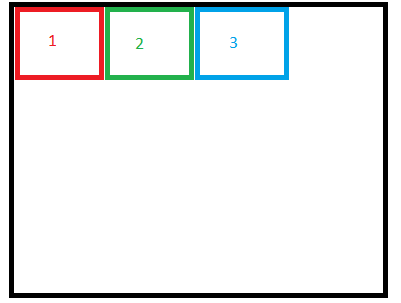
\includegraphics[width=0.4\textwidth]{img/search2}
      \caption{Sequential retrieval of consecutive slices}
  \label{fig:search2}
\end{figure}

\subsubsection*{Deletion}
To the extent of my knowledge, there is no method to remove a single tile from the index by using the rasql language. The only test that can be performed is to to remove the entire collection from the database and to record the amount of time consumed by this operation.

\section{Conclusions and future work}
\label{sec:conclusions}
As stated in the initial project plan, the Hilbert R-tree data structure was implemented in the C++ language with support for n-dimensional objects. This implementation should prove valuable to the community as a whole, and act as a starting point for the integration into rasdaman's indexing mechanism.

The next step was to develop a benchmark for assessing the performance of rasdaman's indexing mechanism. This was accomplished using the benchmarking framework developed by Merticariu in \cite{GM} and extending it with a collection of new queries.

Unfortunately, the research and implementation of the Hilbert R-tree for n-dimensions proved quite involved and accounted for more than 80\% of the time allocated to this project. This lead to the impossibility of successfully achieving the last goal of the project, integrating the Hilbert R-tree into rasdaman. This last task is left for future research. 

\newpage

\newpage
\bibliography{bibliography}

\newpage

\end{document}
